\chapter{Introduction}

Ship handling is the task of precisely controlling a seafaring vessel’s movement using its propulsion and navigation systems. Ships move in a variety of marine environments. From shallow waters of a harbour, a vessel may  navigate vast seas to a port across the ocean. They also navigate inland waterways such as rivers, canals, backwaters and creeks. Handling a ship in such varied environments is the task of a skilled seafarer who controls it's movement precisely with a consideration of environmental forces such as wind, waves and current acting on the ship \parencite{wiki:seamanship}. More recently, developments in offshore wind farming, the oil and gas industry have necessitated regular visits to offshore structures located on continental shelves for construction and maintenance activities. 

Navigation in marine environments just as in aviation requires the navigator to assimilate information of environmental forces at play. In 1955, the US Navy began researching head-up displays (HUD) to reduce complexity of aircraft instrumentation. HUDs were found helpful for piloting and by 1970s, the use of HUDs expanded beyond military aircraft into commercial aviation.

In ships, navigational-aid information has been traditionally presented in display panels placed around the navigator in the ship's bridge. Although aviation and maritime navigation present similar challenges for a navigator, the use of head-up displays is not yet commonplace in the latter. It could be attributable to the maritime industry being a niche sector with a segmented market-space (many small and medium-sized companies), low R\&D intensity and, a conservative attitude towards innovation \parencite{von2014maritime}. Nevertheless, research studies can be found on maritime applications of augmented reality (\cite{hugues2010experimental}, \cite{vasiljevic2011augmented} and, \cite{von2014maritime}). There has been a focus on augmenting vision with real-time information of the environment; potentially helping navigators perform the job more efficiently. For example, overlaying the bridge-view of a ship with route waypoints, distance to next waypoint, local hazards, and navigational aids such as buoys, lighthouses. 

Further, developments in ship instrumentation design over the recent years with newer bridges tending to feature relatively minimal, less-cluttered designs. This design change is also a reflection of increasing automation seeping into industrial processes. The dynamic positioning system for example can be used to automatically position a vessel at a specific location.

%
%, thus making display panels for position, thruster/propeller-related information more redundant than before.\ 

With increasing automation, the need for human-operation will reduce and so will the need to learn to do them manually. Ship simulations systems are currently the \textit{de facto} method of learning ship navigation. Various schools around the world setup simulation centers where generic principles of sea-faring can be learned and practiced. However, there has been little research on the use of mixed reality technologies to create simulation environments for training purposes. This research studies the feasibility of a training method to learn ship navigation in mixed reality environments on-board ships. 
%while also being driven by requirements for customizable instrument panels. 


\subsection{Research Questions}
Ship simulators are used extensively by ship crew for learning, certification and, upkeep of operational skills. Being simulations by nature, they are approximations of the process after all. Training on-board real ships is ideal from the perspective of learning vessel dynamics. It provides for hands-on experience of ship's movement behavior under various weather conditions. Besides, such a training should help get better acquainted with vessel-specific instrumentation. However, it is much more difficult, perhaps even infeasible to set up environments for training purposes on-board real vessels compared to the simulator. This is because training environments in this context involve large physical objects such as ports, natural landscapes, other vessels, etc. For example, an offshore oil platform in the case of dynamic positioning training.   

A system of generating visual perception of a training environment is then desirable. It can be a solution to the non-trivial problem of setting up training environments. If such a system were capable of producing a convincing feeling of the presence of physical objects in the surrounding, it would enable on-board training in real environments enhanced by visuals of virtual objects. 

The following research questions were proposed, with the intention of learning feasibility of using mixed reality technology for training purposes in the maritime sector. 
\textbf{\begin{enumerate}
	\item What are the operational scenarios in which mixed reality training would be useful? 
	\item How is the experience of navigating vessels in mixed reality environment using state-of-the-art see-through display technology?
	\item How effective a tool can mixed reality be for learning ship maneuvering? 
\end{enumerate}}

The remainder of this chapter provides a brief description of the concept of augmented reality before describing the method of research used in this study.

\section{Augmented Reality}
\label{sec:augreal}
Augmented reality refers to the merging of virtual and real worlds in which physical and digital objects co-exist and interact in real time. In this realm, distinctions have been made between various types of applications based on the amount of virtual content in the mix. \cite{milgram1995augmented} drew up a continuum (figure \ref{fig:mixedrealitycontinuum}) characterising different mixed reality environments. Completely real and completely virtual environments bring up far ends of the continuum with different levels of virtuality in between. 

\begin{figure}
	\centering
	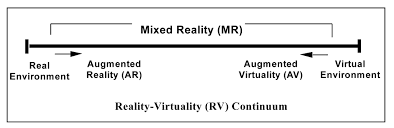
\includegraphics[width=0.75\linewidth]{mixedrealitycontinuum}
	\caption{Mixed Reality Continuum (Source: \cite{milgram1995augmented})}
	\label{fig:mixedrealitycontinuum}
\end{figure}

Virtual reality lies in the extreme right of this spectrum. Here, user's perception of reality is influenced to create the feeling of immersion in a completely virtual world. It is a specific type of mixed reality featuring entirely digital visuals and virtual environments. Driven by the gaming industry, this type of mixed reality is more technologically advanced as of this writing.

Augmented reality on the other hand refers to systems that feature predominantly real environments whose perception may be augmented with information not readily available to the user. It is also used in context of 3D visualizations of designs in real world spaces. In a definitive paper on augmented reality, \textcite{azuma1997survey} identified the technology to have the following three characteristics: 
\begin{enumerate}
	\item It combines real and virtual 
	\item Is interactive in real time
	\item Is registered in three dimensions
\end{enumerate} 

\begin{figure}
	\centering
	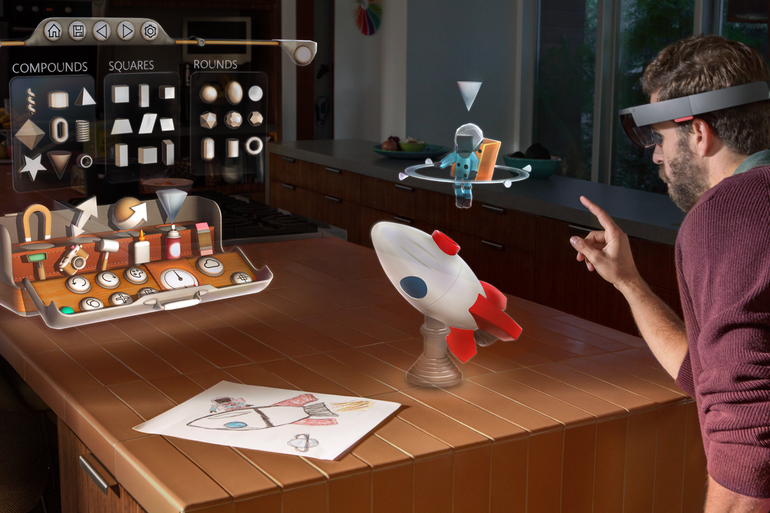
\includegraphics[width=\linewidth]{hololensAR}
	\caption{Conceptual depiction of augmented reality used in design}
	\label{fig:augreal}
\end{figure}

%Further, some factors have been identified that help distinguish between different mixed reality systems: extent of world knowledge (whether the augmentation takes place in a modeled world or not), reproduction fidelity (quality of display of the real/virtual objects) and extent of presence metaphor (extent to which user feels they are present in the displayed scene themselves). A detailed description of mixed reality displays and differences in their characteristics can be found in \cite{milgram1995augmented}. 

In general terms, mixed reality is an emerging technology which can be used to display virtual objects merged with real world views. It has been found to be useful in job scenarios that require execution of complex tasks. One use case that has been explored in the real-world is assembly and maintenance of equipment. During an operation, overlaying 3-D virtual job-support guides on see-through images of actual equipment obviates the need to look away in order to refer to a manual. A study on the application of augmented reality found that 3-D virtual guides help users perform ship building and maintenance tasks in almost half the usual time \parencite{henderson2011exploring}.



\section{Research Method}
A research method devised by \cite{neerincx2008situated} called situated cognitive engineering was used in this study. This method separates a human-computer interaction research into three different phases namely derive, specify and evaluate. Accordingly, this report has been structured to describe the three phases of this research outlined by sCE. Chapter 2 named Foundation first describes so-called operational demands that define requirements of the problem at an abstract level. It goes on to describe existing knowledge of human anatomical factors that can be leveraged in designing a solution to the problem. The chapter ends with a survey of possible technological solutions, stating also their strengths and weaknesses. Chapter 3 named Specification sketches a real-life scenario in which the artifact could possibly be used. It lists formal requirements for the software system and makes claims about consequences of its use. Chapter 4 named Evaluation describes the artifact that was developed, an experiment designed to test the claims and, discusses result and conclusion of the experiment. 

\begin{figure}
	\centering
	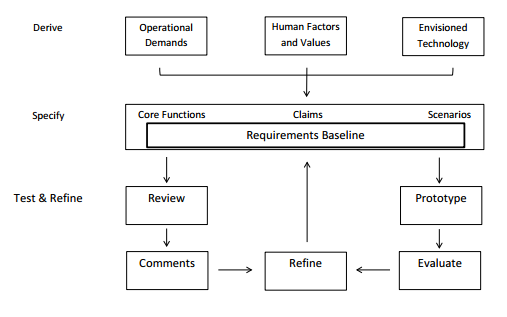
\includegraphics[width=0.90\linewidth]{situatedcognitive}
	\caption{Situated Cognitive Engineering Method \parencite{neerincx2008situated}}
	\label{fig:augreal}
\end{figure}
